The interface of our System is thought to be used via mobile app, because all the functionality make sense only in a \textit{movable} context (meaning, such that the user can do them anywhere they have an internet connection).

We will now list some of the user interfaces thought for \textit{Travlendar+}":

% login %
\begin{figure}[h]
	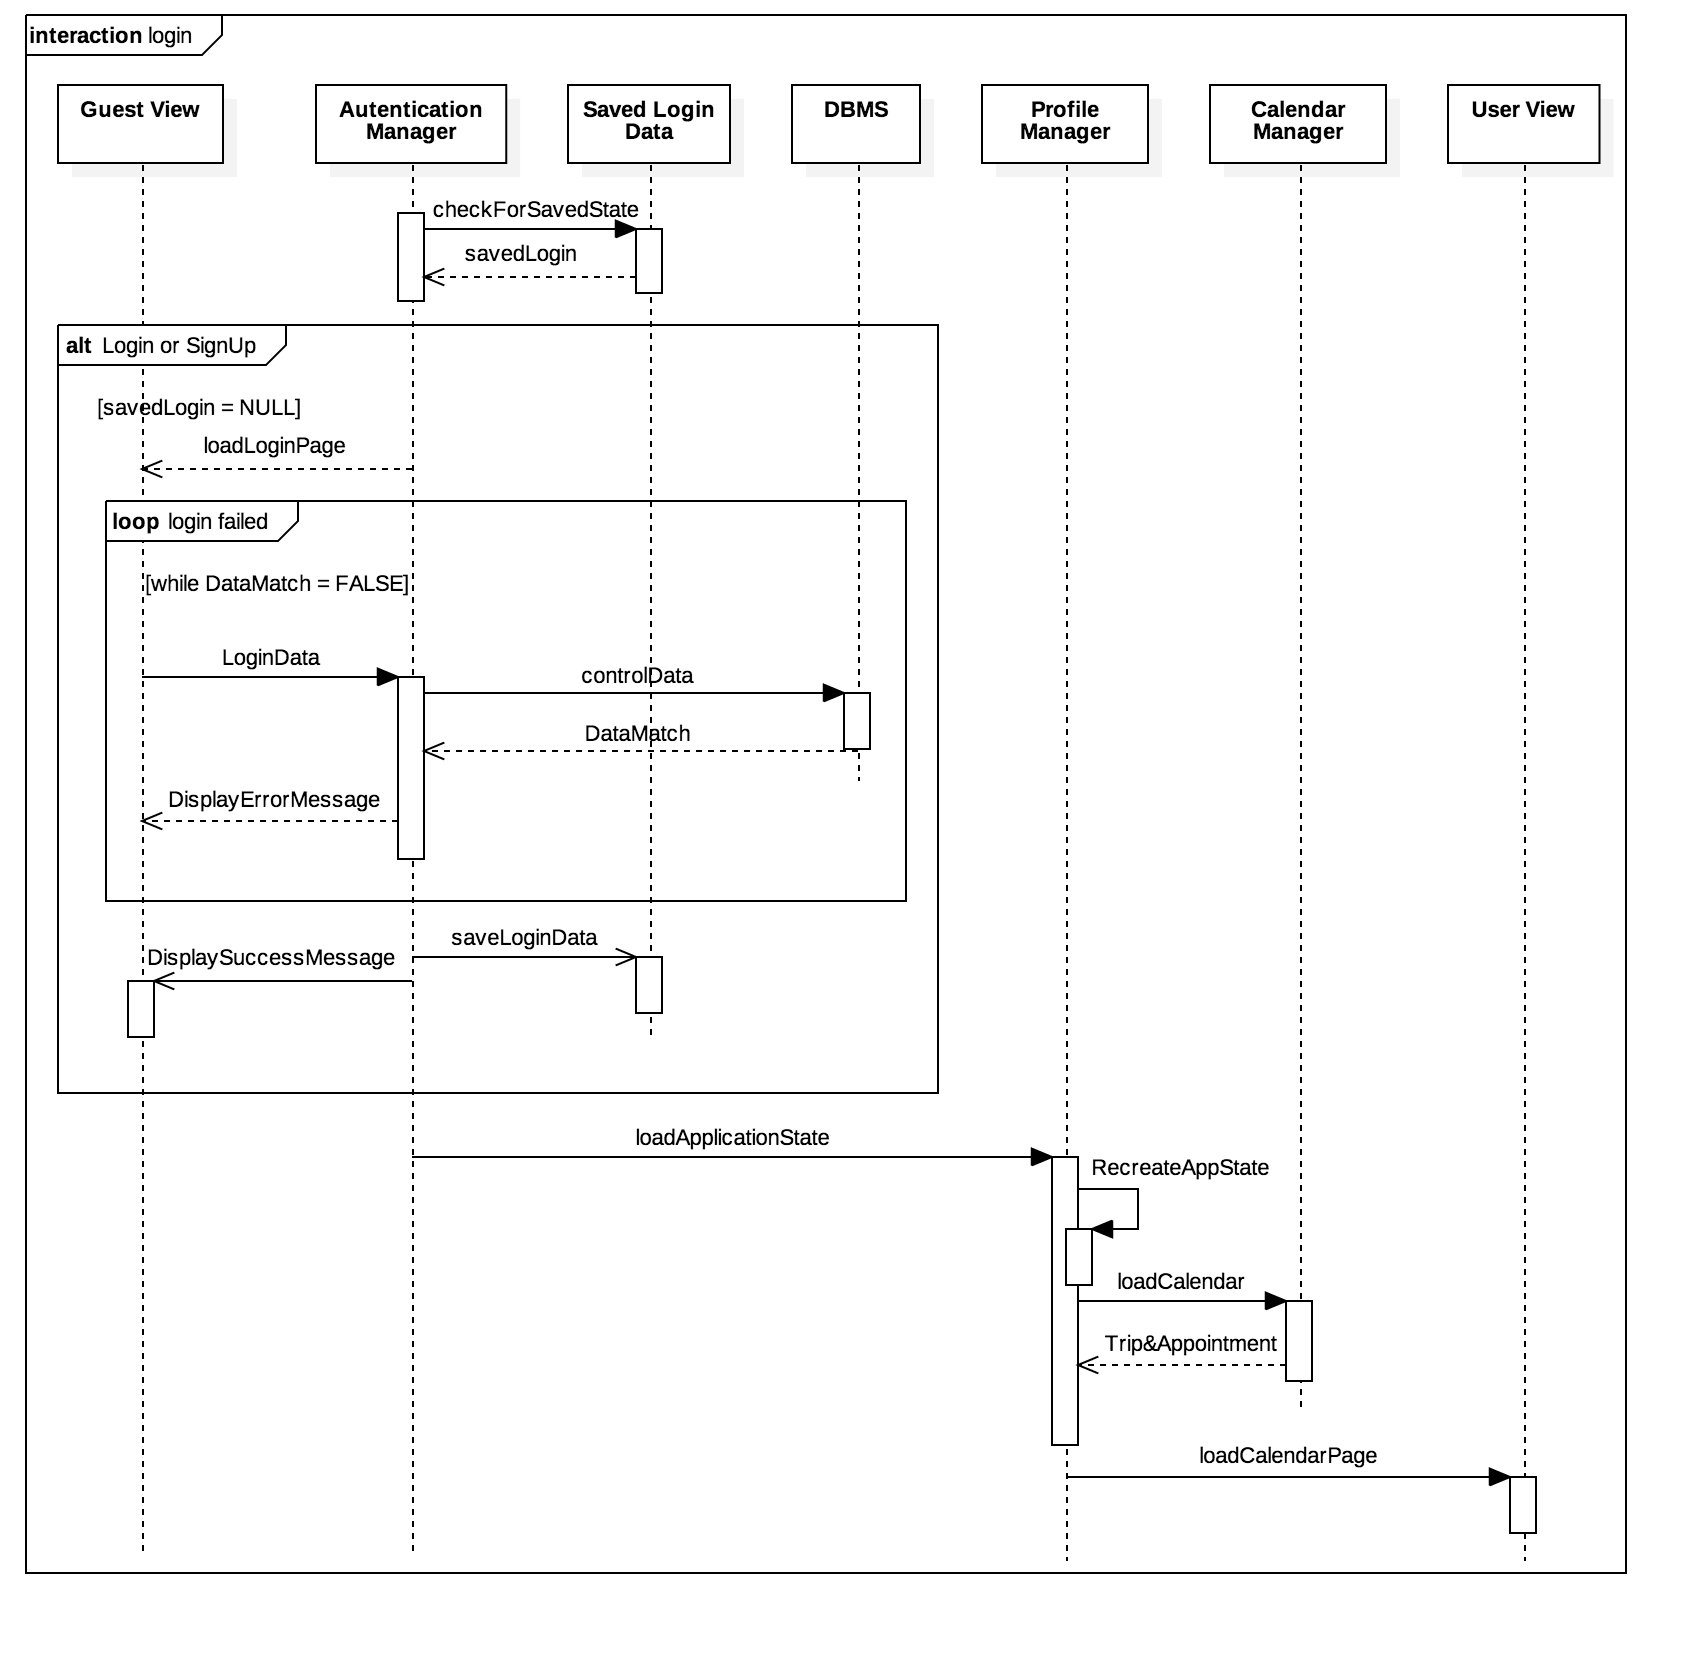
\includegraphics[width=5cm, height=9.5cm]{mockup/login}
	\centering
	\caption{Login Page.}
	\label{fig:login}
\end{figure}
As mentioned before, a \textit{Guest} or a \textit{non logged User} will encounter page showed in figure \ref{fig:login}, and he will never enter into the app until he completes the Registration or the Login procedures (see sections \ref{register_useCase} and \ref{login_useCase}).
% home page %

\begin{figure}[H]
	\begin{subfigure}{0.5\textwidth}
		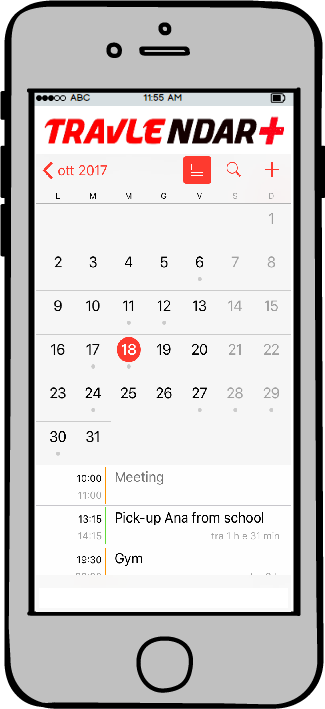
\includegraphics[width=5cm, height=9.5cm]{mockup/homepageMonth} 
		\centering
		\caption{Home Page in Monthly view.}
		\label{fig:homePage_Month}
	\end{subfigure}
	\begin{subfigure}{0.5\textwidth}
		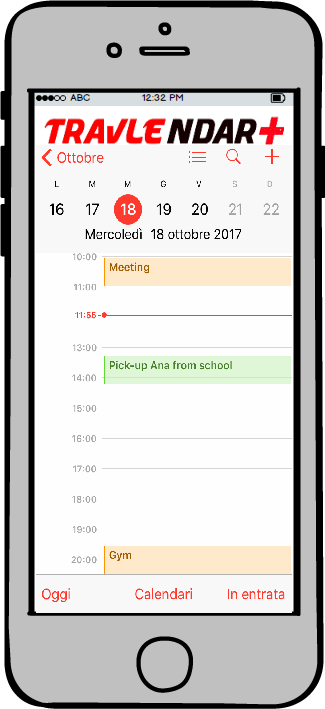
\includegraphics[width=5cm, height=9.5cm]{mockup/homepageDaily} 
		\centering
		\caption{Home Page in Daily view.}
		\label{fig:homePage_Day}
	\end{subfigure}
	\caption{Samples of view events.}
\end{figure}
The user can use two different views to manage events in his homepage. Theese are rappresented in figure 2. On the left the application shows monthly view, on the right the daily view. Thus user will modify the scheduling in a simple way by clicking on the events

% create Event %
\begin{figure}[H]
	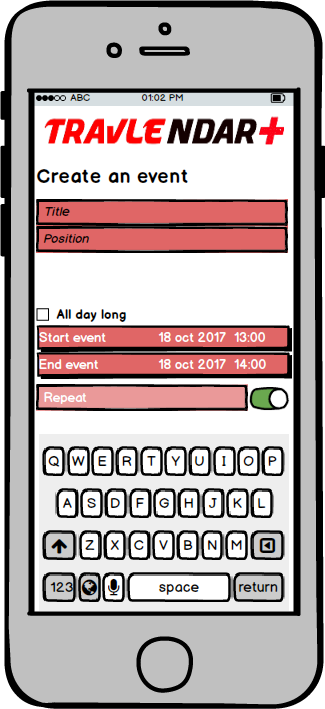
\includegraphics[width=5cm, height=9.5cm]{mockup/createAnEvent}
	\centering
	\caption{Create an Appointment page.}
	\label{fig:createEvent}
\end{figure}
When the user wants to creates an event, he has to use this interface of the application. In fact figure 3 shows what user can choose his preferences about the event.\\

% travel Logic %
The application computes the possible solutions to reach a certain event based on the starting position. These are displayed on the screen of the user's smartphone as shown in Figure 4a. The user must choose the preferred solution to see the details. It may happen that the solution contains buy tickets (fig 4b) or hire cars (fig 4c). Clicking on the corresponding buttons will open the corresponding application.

\begin{figure}[H]
	\caption{Samples of the Travel logic module.}
	
	\begin{subfigure}{0.5\textwidth}
		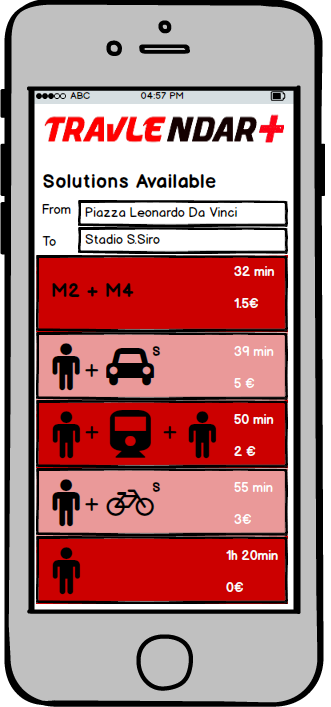
\includegraphics[width=5cm, height=9.5cm]{mockup/solutions} 
		\centering
		\caption{Solutions found for an Event view.}
		\label{fig:solutions}
	\end{subfigure}
	\begin{subfigure}{0.5\textwidth}
		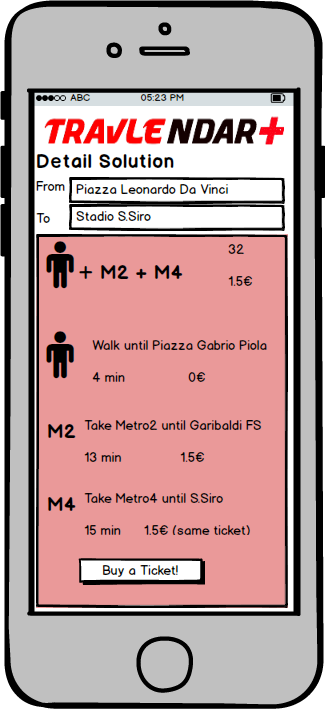
\includegraphics[width=5cm, height=9.5cm]{mockup/buyATicket} 
		\centering
		\caption{Buy a public transportation ticket view.}
		\label{fig:buyTicket}
	\end{subfigure} \\
	\begin{subfigure}{\linewidth}
		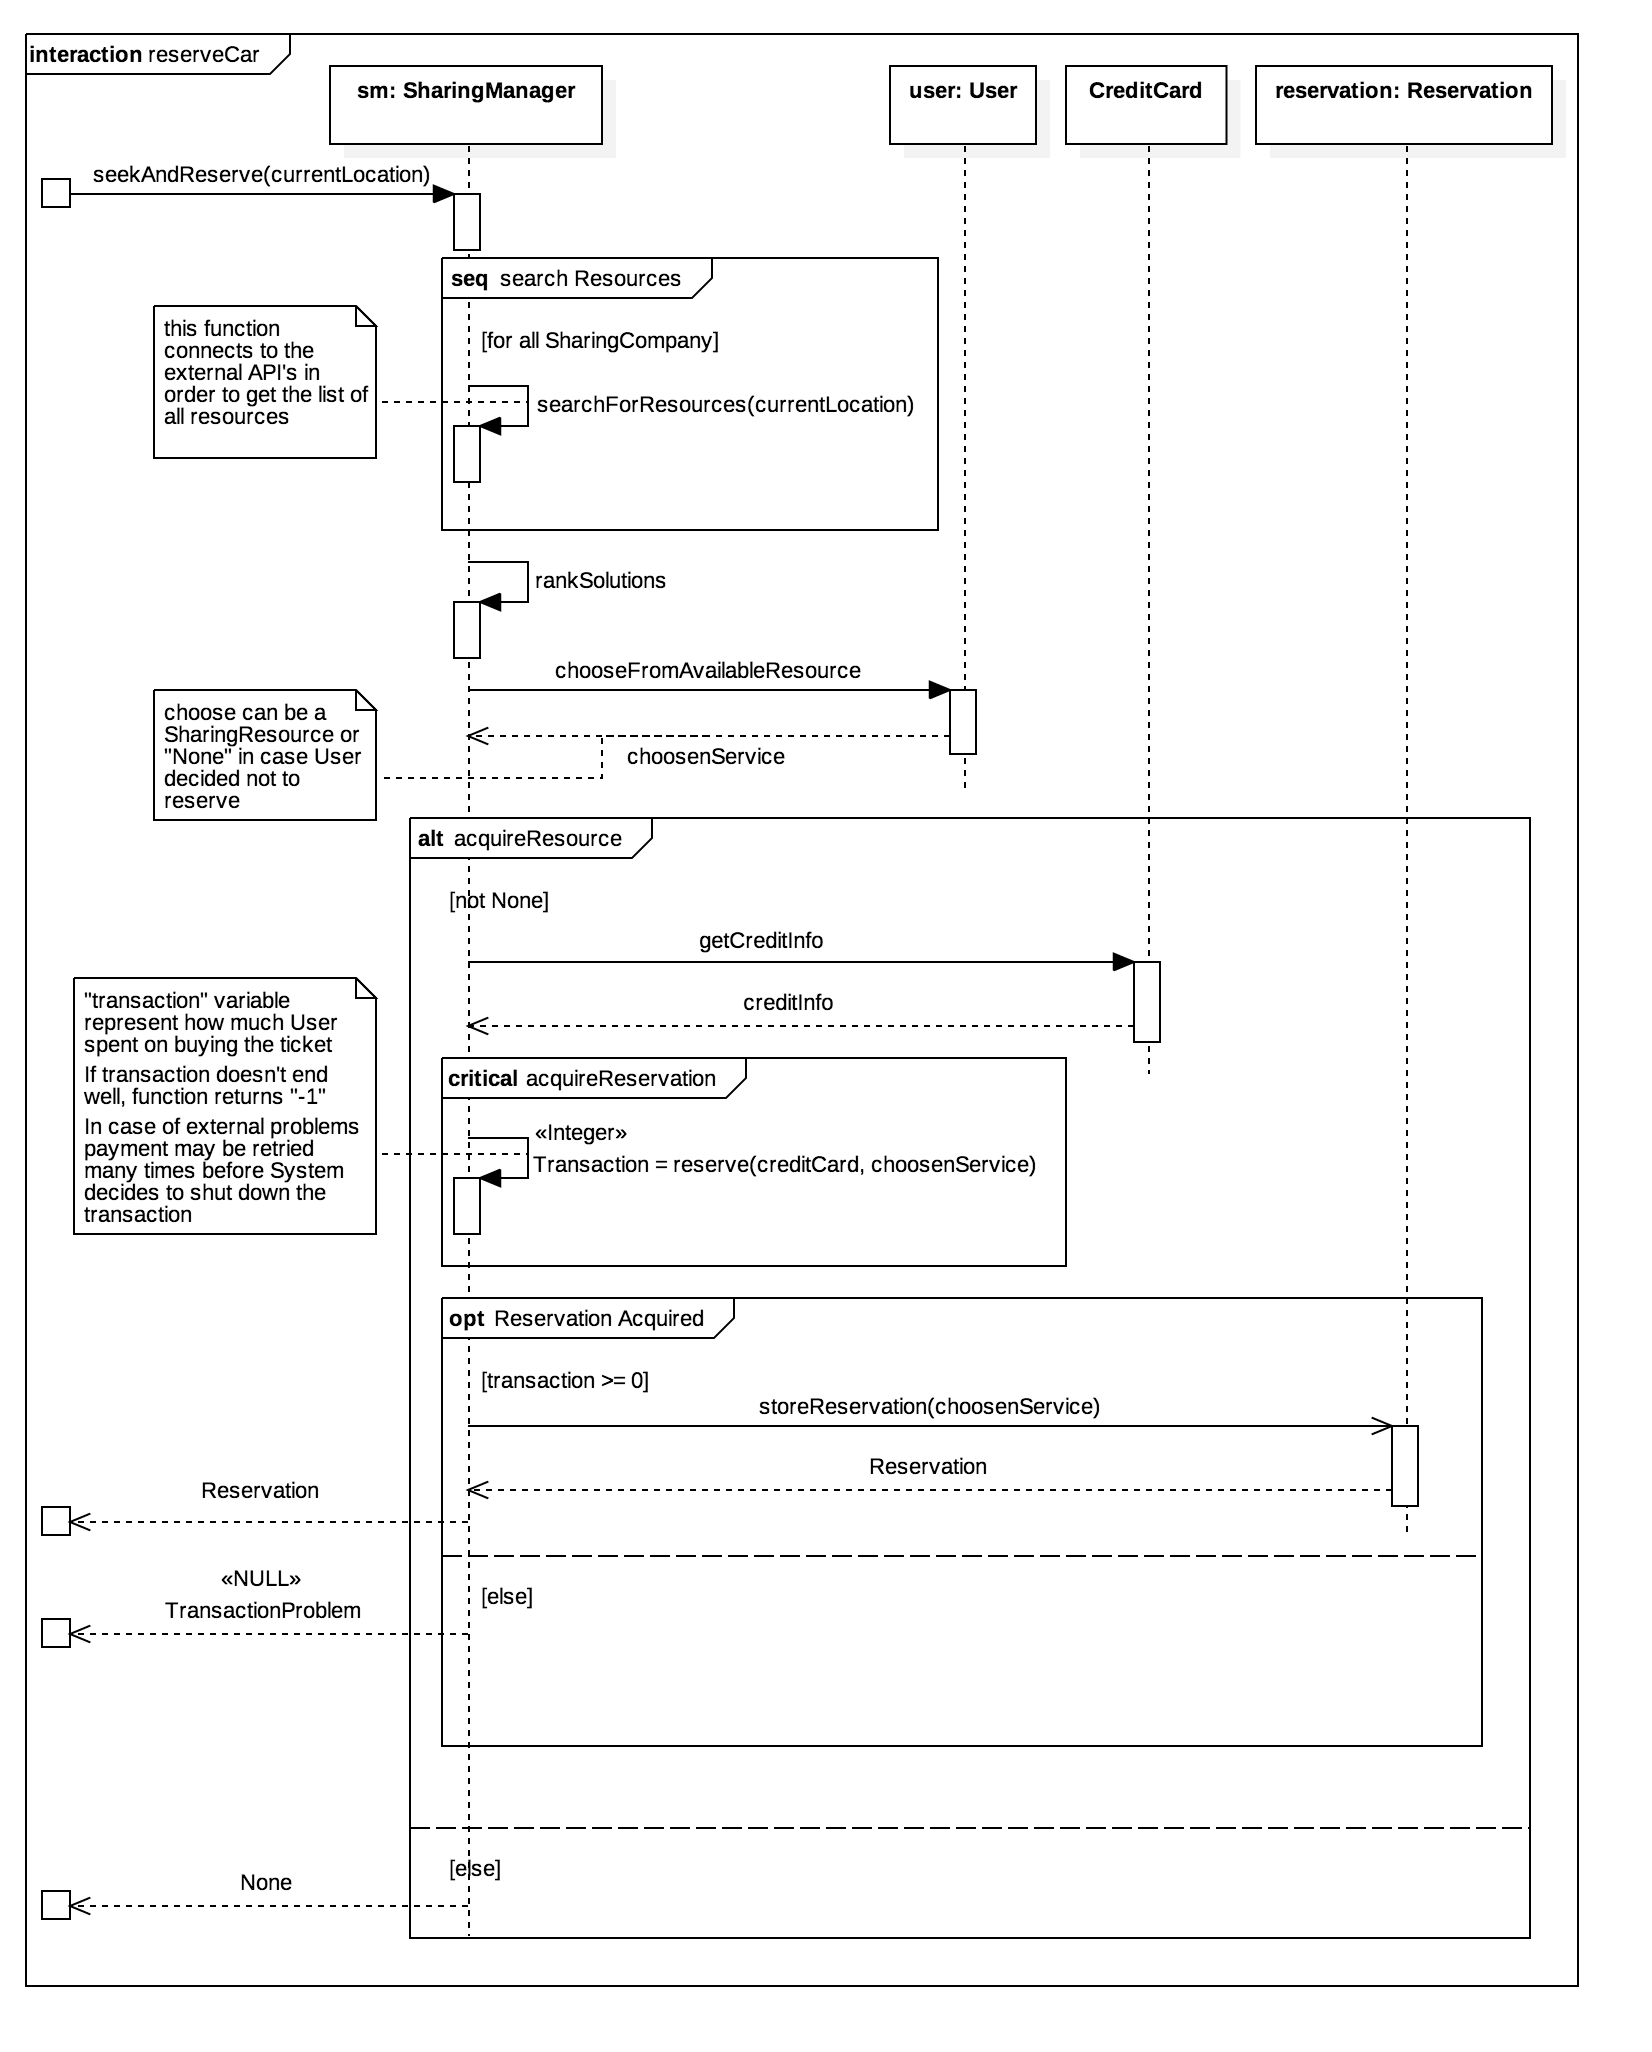
\includegraphics[width=5cm, height=9.5cm]{mockup/reserveCar} 
		\centering
		\caption{Reserve a Sharing service resource view.}
		\label{fig:reserveCar}
	\end{subfigure}

	\label{fig:travelLogic}
\end{figure}